\documentclass[tikz, border=5pt]{standalone}
\usepackage{helvet}
\renewcommand{\familydefault}{\sfdefault}
\usetikzlibrary{shapes.geometric, arrows.meta, positioning, calc}

\begin{document}
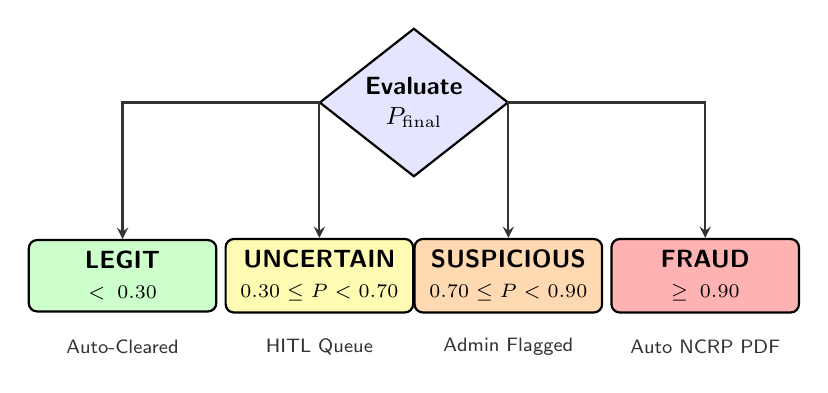
\begin{tikzpicture}[
    process/.style={rectangle, rounded corners=3pt, draw=black, thick, align=center, font=\small\bfseries, text=black, inner sep=4pt, minimum height=0.8cm},
    decision/.style={diamond, draw=black, thick, fill=blue!10, text=black, align=center, inner sep=0pt, font=\small\bfseries, minimum width=2.4cm, minimum height=1.4cm},
    arrow/.style={->, thick, >=stealth, draw=black!80}
]

\node[decision] (eval) at (0, 0) {Evaluate\\$P_{\mathrm{final}}$};

\node[process, fill=green!20, text width=2.1cm] (legit) at (-3.7, -2.2) {LEGIT\\{\scriptsize $< 0.30$}};
\node[process, fill=yellow!30, text width=2.1cm] (uncertain) at (-1.2, -2.2) {UNCERTAIN\\{\scriptsize $0.30 \leq P < 0.70$}};
\node[process, fill=orange!30, text width=2.1cm] (susp) at (1.2, -2.2) {SUSPICIOUS\\{\scriptsize $0.70 \leq P < 0.90$}};
\node[process, fill=red!30, text width=2.1cm] (fraud) at (3.7, -2.2) {FRAUD\\{\scriptsize $\geq 0.90$}};

\draw[arrow] (eval) -| (legit.north);
\draw[arrow] (eval) -| (uncertain.north);
\draw[arrow] (eval) -| (susp.north);
\draw[arrow] (eval) -| (fraud.north);

\node[font=\scriptsize, color=black!80, align=center] at (-3.7, -3.1) {Auto-Cleared};
\node[font=\scriptsize, color=black!80, align=center] at (-1.2, -3.1) {HITL Queue};
\node[font=\scriptsize, color=black!80, align=center] at (1.2, -3.1) {Admin Flagged};
\node[font=\scriptsize, color=black!80, align=center] at (3.7, -3.1) {Auto NCRP PDF};

\end{tikzpicture}
\end{document}
